\documentclass[22pt,a4paper]{article}
\usepackage[a4paper,margin=6mm]{geometry}
\usepackage{amsmath,amsthm,amssymb}
\usepackage{amsbsy}
\usepackage{hyperref}
\usepackage[capitalise,nameinlink,noabbrev]{cleveref}
\usepackage[utf8x]{inputenc}
\usepackage{textcase}
\usepackage{graphicx}
\usepackage{fontspec} 
\usepackage{titlesec}
\setmainfont{Gotham}

\crefname{equation}{}{}


% Section Spacing
\titlespacing*{\section}
{0pt}{5.5ex plus 1ex minus .2ex}{4.3ex plus .2ex}
\titlespacing*{\section}
{0pt}{20ex}{5ex}
% END Section Spacing

\linespread{1.7}
\theoremstyle{definition}
\newtheorem{definition}{Ορισμός}[section]
\newtheorem{theorem}{Θεώρημα}[section]
\title{%
  \large Ανάλυση Ανεξάρτητων, Θετικών Συνιστώσων \\
  \vspace{5mm}
  \small Αρχές και Μέθοδοι Μηχανικής Μάθησης \\
  \vspace{5mm}
  \footnotesize Σημείωσεις στις σημείωσεις του κ. Διαμαντάρα}
\date{}

\begin{document}

\maketitle

\section*{Ανεξάρτητοι Παράγοντες}

Από το PCA γνωρίζουμε ότι οι παράγοντες $y_i$ είναι \textbf{Στατιστικά Ασυσχέτιστοι} μεταξύ τους. Δηλαδή ισχύει:
\begin{equation}
  \boxed{E \{y_i y_j\} = 0, i \neq j }
\end{equation}
Αλλά, \\
Σε κάποιες εφαρμογές είναι σωστότερο να υποθέσουμε ότι οι \textbf{κρυφοί παράγοντες} είναι \textbf{στατιστικά ανεξάρτητοι}, δηλαδή έχουμε:
\begin{equation}
  \boxed{
    p(y_i,y_j) = p(y_i) * p(y_j)
  }
\end{equation}
Και αυτό γιατί η ανεξαρτησία είναι \textbf{πιο ισχυρή} από την έλλειψη συσχέτισης:
\begin{equation}
  \boxed{
    y_i,y_j \text{Ανεξάρτητοι} \Rightarrow y_i,y_j \text{Ασυσχέτιστοι}
  }
\end{equation}
Δηλαδή οι ασυσχέτιστοι \textbf{δεν σημαίνει} απαραίτητα ότι είναι και ανεξάρτητοι.
\begin{equation}
  \boxed{
    y_i,y_j \text{Ανεξάρτητοι} \nLeftarrow y_i,y_j \text{Ασυσχέτιστοι}
  }
\end{equation}

\section*{Πως μπορεί να χρησιμοποιηθεί}

Έστω ότι υπάρχουν 2 παρουσιαστές σε μια σκηνή με 1 μικρόφωνο ο καθένας.
Δυστυχώς, επειδή είναι πολύ κοντά, \textbf{οι φωνές και των 2 απορροφούνται και από τα 2 μικρόφωνα!} Με το ICA, θα μπορούσαμε αφού έχουμε τα μπλεγμένα δεδομένα, να τα \textbf{ξεμπλέξουμε και να ξεχωρίσουμε τις 2 φωνές.}


\section*{Ανάλυση Ανεξαρτήτων Συνιστώσων}

\begin{itemize}
  \item \underline{Δεδομένα}:
        \begin{itemize}
          \item Παρατηρήσεις: $\pmb{x}(1),...,\pmb{x}(N) \in \mathbb{R}^n $
          \item Δεν χρησιμοποιούνται στόχοι $t$ (Χωρίς Επίβλεψη)
          \item Πλήθος παραγόντων $n$
        \end{itemize}
  \item \underline{Πρόβλημα}: Βρες τον πίνακα $\pmb{F} \in \mathbb{R}^n*n$ έτσι ώστε οι παράγοντες $y_i = \pmb{f}^T_i \pmb{x}$ να είναι στατιστικά ανεξάρτητοι μεταξύ τους.
        \begin{itemize}
          \item $\pmb{f}^T_i$ οι γραμμές του $\pmb{F}$
        \end{itemize}
  \item \underline{Παρατήρηση}: Αν θέσουμε
        \begin{itemize}
          \item $\pmb{W} = \pmb{F}^{-1}$
          \item $\pmb{y} = \pmb{Fx}$
          \item τότε $\pmb{x = Wy = w_1}y_1+...+\pmb{w}_n y_n$
        \end{itemize}
\end{itemize}

\begin{figure}[h]
  \caption{Μοντέλο ICA}
  \centering
  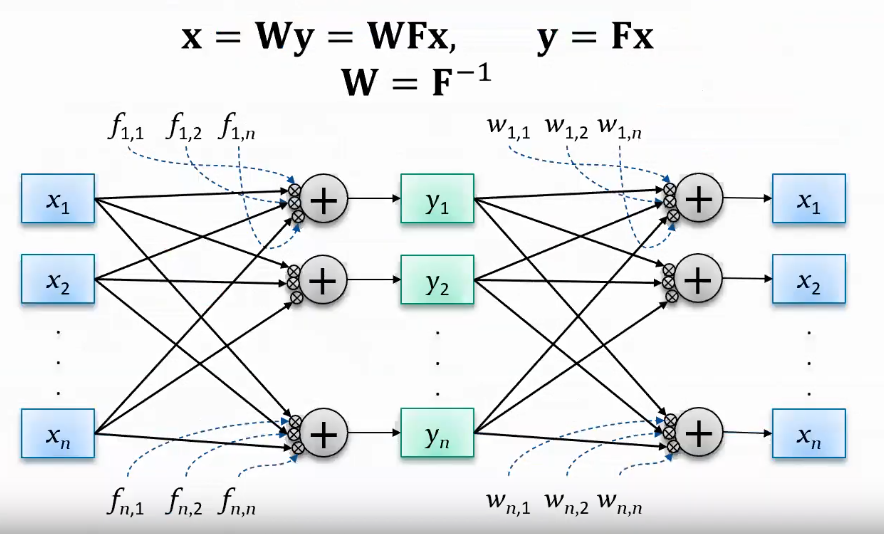
\includegraphics[width=0.70\textwidth]{./images/ica_model.jpg}
\end{figure}


\section*{Συσσωρεύτριες (cumulants)}


Οι Συσσωρεύτριες είναι συναρτήσεις αντίθεσης.
\begin{definition}
  Μια συσσωρεύτρια $k$ τάξης μιας τυχαίας μεταβλητής $x$ ορίζεται ως
  \begin{equation}
    \boxed{
      c_k(x) = (-j)^k \frac{d^k\phi_x(\omega)}{d\omega^k}
    }
  \end{equation}

\end{definition}
Όπου $\phi_x(\omega) = lnE\{e^{j \omega x}\}$ \\

Και πρακτικά έχουμε:
\begin{itemize}
  \item $c_1 = E\{x\}$
  \item $c_2 = E\{x^2\}$ (διακύμανση)
  \item $c_3 = E\{x^3\}$
  \item $c_4 = E\{x^4\} - 3E\{x^2\}$ (κύρτωση, αρκετά χρήσιμη)
  \item ...κλπ
\end{itemize}

\section*{Προεπεξεργασία Δεδομένων}


1. \underline{Αφαίρεση μέσου όρου}: $\pmb{x\Rightarrow x': }E \{\pmb{x'}\} = 0 $ \\
2. \underline{Λεύκανση}: $\pmb{x'\Rightarrow\bar{x}:}E\{\pmb{\bar{x}\bar{x}^T\}=I}$
\begin{definition}
  Λεύκανση ονομάζεται η τετραγωνοποίηση διαγράμματος μιας ομάδας δεδομένων.
\end{definition}

\begin{figure}[h]
  \caption{Παράδειγμα}
  \centering
  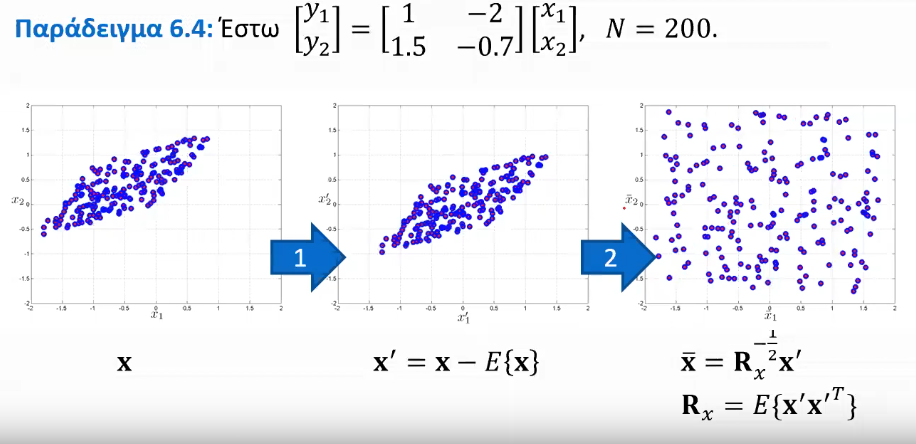
\includegraphics[width=0.70\textwidth]{./images/ica_example.png}
\end{figure}

\section*{Εξαγωγή ενός παράγοντα}

Έστω για κάποιο $\pmb{f}: z(k) = \pmb{f^T x(k)}$ \\
θα έχουμε $z(k) = \pmb{f^T Wy}(k)$ \\
όπου  $\pmb{f^T} = \pmb{v^T}$ \Rightarrow $z(k) = \pmb{v^T y(k)}$

\begin{theorem}
  Αν οι παράγοντες δεν είναι Γκαουσσανές τυχαίες μεταβλητές, τότε η μεγιστοποίηση της κύρτωσης $J\pmb{(f)} = |c_4(z)| $ υπό τον περιορισμό $c_2(z)=1$ επιτυγχάνεται για \\
  $\pmb{v}$ = [0 0 ... 0 α 0 ... 0]
\end{theorem}


\section*{Περιορισμοί}

\begin{itemize}
  \item Χάνεται η σειρά των παραγόντων, δηλαδή οι εκτιμώμενοι παράγοντες $y_i$ μπορεί να είναι ανακατωμένοι.
  \item Οι παράγοντες μπορεί να εξαχθούν με αυθαίρετη κλιμάκωση. Πιθανή \textbf{αλλαγή προσήμου}.
  \item Κάθε ανάλυση ICA σε ίδια δεδομένα μπορεί να εξάγει παράγοντες με διαφορετική σειρά και κλιμάκωση.
\end{itemize}

\section*{PCA εναντίον ICA}

\begin{center}
  \begin{tabular}{|p{50mm}|p{40mm}|p{40mm}|}
    \hline
    Ζουμί                         & PCA                                         & ICA                                    \\
    \hline
    Πλήθος παραγόντων(συνιστώσων) & m ($\leq$ διάσταση διανύσματος παρατήρησης) & n (= διάσταση διανύσματος παρατήρησης) \\
    \hline
    Σχέση παραγόντων              & Ασυσχέτιστοι                                & Ανεξάρτητοι                            \\
    \hline
    Συνάρτηση Κόστους             & Μέσο τετραγωνικό σφάλμα                     & Συναρτήσεις αντίθεσεις                 \\
    \hline
  \end{tabular}
\end{center}

\end{document}